\documentclass[10pt,utf8,compress,xcolor=dvipsnames]{beamer}
\usefonttheme{professionalfonts}
\usepackage[greek,english]{babel}
%\usefonttheme{}
%\usetheme{Hannover}
\usetheme{Warsaw}
\usepackage{graphicx}
\usepackage{amsmath}
\usepackage{slashed}
\setbeamercolor{background canvas}{bg=white}
\setbeamertemplate{navigation symbols}{}
\usepackage{float}

\setbeamertemplate{headline}{}

\usepackage[absolute,overlay]{textpos}
\usepackage{rotating}
\usepackage{multicol}
\usepackage{ifthen}
\usepackage[dvipsnames]{xcolor}
\usepackage{tikz}


%Define color environments:

\newenvironment{DK}[1]{{\color{gray}Commend from D: #1}}

\newenvironment{DKnew}[1]{{\color{blue}NEW from D: #1}}

\newenvironment{DKres}[1]{{\color{BrickRed}RESTRUCTURED from D: #1}}




\newcommand{\dint}{  \displaystyle \int }
%%%%%%%%%%%%%%%%%%%%%%%%%%%%%%%%%%%%%%%%%%
\newcommand{\ie}{{\em i.e.} }
\newcommand{\eg}{{\em e.g.} }
\newcommand{\GeV}{{\rm GeV}}
\newcommand{\TeV}{{\rm TeV}}
\newcommand{\MeV}{{\rm MeV}}
\newcommand{\keV}{{\rm keV}}

\newcommand{\rhs}{RHS }
\newcommand{\lhs}{LHS }


\newcommand{\geff}{ g_{\rm eff} }
\newcommand{\heff}{ h_{\rm eff} }
 
\newcommand{\Ham}{ \mathcal{H} }
 
\newcommand{\thetamax}{ \theta_{\rm max}{} }

 
\newcommand{\thetai}{ \theta_{\rm ini}{} }

\newcommand{\fa}{ f_{\alpha}{} }
 
\newcommand{\ti}{ t_{\rm ini}{} }
 
\newcommand{\Ri}{ R_{\rm ini}{} }


\newcommand{\tosc}{ t_{\rm osc}{} }

\newcommand{\Omegai}{ \Omega_{\rm ini} }
 
\newcommand{\ma}{ m_\alpha{} }

\newcommand{\Lint}{ \mathcal{L}_{\rm int} }


\newcommand{\vev}[1]{\langle #1 \rangle}
\newcommand{\Bvev}[1]{\Bigg\langle #1 \Bigg\rangle}
\newcommand{\bvev}[1]{\Big\langle #1 \Big\rangle}




\newcommand{\lrb}[1]{\left( #1 \right)}
\newcommand{\lrsb}[1]{\left[ #1 \right]}
\newcommand{\lrBigb}[1]{\Big( #1 \Big)}
\newcommand{\lrBigsb}[1]{\Big[ #1 \Big]}
\newcommand{\lrBiggb}[1]{\Bigg( #1 \Bigg)}
\newcommand{\lrBiggsb}[1]{\Bigg[ #1 \Bigg]}

\newcommand{\lrBigcb}[1]{\Big\{ #1 \Big\}}
\newcommand{\lrBiggcb}[1]{\Bigg\{ #1 \Bigg\}}
%%%%%%%%%%%%%%%%%%%%%%%%%%%%%%%%%%%%%%%%%

%%%%%%%%%%%%%%%%%%%%%%%%%%%%%%%%%%%%%%%%%%%%%%%%%%%--Begin_refs--%%%%%%%%%%%%%%%%%%%%%%%%%%%%%%%%%%%%%%%%%%%%%%%%%%%%%%%%%%%%%%%%%%%%%%
\newcounter{NumArgs}

%Define reference to an arbitrary number of equations (\eqs{label_1,label_2....,label_n} will show eqs. ref_1, ref_2, ..., and ref_n)
\newcommand{\eqs}[1]{\setcounter{NumArgs}{0}\foreach\i in{#1}{\stepcounter{NumArgs}}%
\ifthenelse{\equal{\theNumArgs}{1}}{eq.~(\ref{#1})}%
{\ifthenelse{\equal{\theNumArgs}{2}}%
{eqs.~\foreach\i[count=\q]in{#1}{\ifthenelse{\equal{\q}{\theNumArgs}}{and (\ref{\i})}{(\ref{\i})~}}}%
{eqs.~\foreach\i[count=\q]in{#1}{\ifthenelse{\equal{\q}{\theNumArgs}}{and (\ref{\i})}{(\ref{\i}),~}}}}}


%Define reference to an arbitrary number of equations (\Eqs{label_1,label_2....,label_n} will show Eqs. ref_1, ref_2, ..., and ref_n)
\newcommand{\Eqs}[1]{\setcounter{NumArgs}{0}\foreach\i in{#1}{\stepcounter{NumArgs}}%
\ifthenelse{\equal{\theNumArgs}{1}}{Eq.~(\ref{#1})}%
{\ifthenelse{\equal{\theNumArgs}{2}}%
{Eqs.~\foreach\i[count=\q]in{#1}{\ifthenelse{\equal{\q}{\theNumArgs}}{and (\ref{\i})}{(\ref{\i})~}}}%
{Eqs.~\foreach\i[count=\q]in{#1}{\ifthenelse{\equal{\q}{\theNumArgs}}{and (\ref{\i})}{(\ref{\i}),~}}}}}


%Define reference to an arbitrary number of labels (\REF{label_1,label_2....,label_n} will show ref_1, ref_2, ..., and ref_n)
\newcommand{\refs}[1]{\setcounter{NumArgs}{0}\foreach\i in{#1}{\stepcounter{NumArgs}}%
\ifthenelse{\equal{\theNumArgs}{1}}{(\ref{#1})}%
{\ifthenelse{\equal{\theNumArgs}{2}}%
{\foreach\i[count=\q]in{#1}{\ifthenelse{\equal{\q}{\theNumArgs}}{and (\ref{\i})}{(\ref{\i})~}}}%
{\foreach\i[count=\q]in{#1}{\ifthenelse{\equal{\q}{\theNumArgs}}{and (\ref{\i})}{(\ref{\i}),~}}}}}



%Define reference to an arbitrary number of figs (\Figs{label_1,label_2....,label_n} will show ref_1, ref_2, ..., and ref_n)
\newcommand{\Figs}[1]{\setcounter{NumArgs}{0}\foreach\i in{#1}{\stepcounter{NumArgs}}%
\ifthenelse{\equal{\theNumArgs}{1}}{Fig.~(\ref{#1})}%
{\ifthenelse{\equal{\theNumArgs}{2}}%
{Figs.~\foreach\i[count=\q]in{#1}{\ifthenelse{\equal{\q}{\theNumArgs}}{and (\ref{\i})}{(\ref{\i})~}}}%
{Figs.~\foreach\i[count=\q]in{#1}{\ifthenelse{\equal{\q}{\theNumArgs}}{and (\ref{\i})}{(\ref{\i}),~}}}}}




%Define reference to an arbitrary number of "general reference" (\Gen{message}{label_1,label_2....,label_n} will show message.(ref_1), (ref_2), ..., and (ref_n)
\newcommand{\Gen}[2]{\setcounter{NumArgs}{0}\foreach\i in{#2}{\stepcounter{NumArgs}}%
	\ifthenelse{\equal{\theNumArgs}{1}}{#1.~(\ref{#2})}%
	{\ifthenelse{\equal{\theNumArgs}{2}}%
		{#1.~\foreach\i[count=\q]in{#2}{\ifthenelse{\equal{\q}{\theNumArgs}}{and (\ref{\i})}{(\ref{\i})~}}}%
		{#1.~\foreach\i[count=\q]in{#2}{\ifthenelse{\equal{\q}{\theNumArgs}}{and (\ref{\i})}{(\ref{\i}),~}}}}}


%%%%%%%%%%%%%%%%%%%%%%%%%%%%%%%%%%%%%%%%%%%%%%%%%%%--End_refs--%%%%%%%%%%%%%%%%%%%%%%%%%%%%%%%%%%%%%%%%%%%%%%%%%%%%%%%%%%%%%%%%%%%%%%




\setbeamercolor{structure}{fg=red!80!black}
\setbeamercolor{section in head/foot}{fg=yellow, bg=black!80!red}%purple!30!black}
\setbeamercolor{frametitle}{fg=yellow!90!black}
\setbeamertemplate{footline}{
%	\hspace{0.5cm}\vspace*{5cm}
%	\begin{multicols}{2}
%		\setbeamercolor{section in head/foot}{fg=yellow, bg=blue!100!black}%purple!30!black}
%			\begin{beamercolorbox}[wd=0.6\textwidth,ht=2.25ex,dp=0.9ex,center]{section in head/foot}%
%				\insertframenumber/\inserttotalframenumber
%			\end{beamercolorbox}
%		\columnbreak
%		\setbeamercolor{section in head/foot}{fg=yellow, bg=blue!50!black}%purple!30!black}
%			\begin{beamercolorbox}[wd=0.6\textwidth,ht=2.25ex,dp=0.9ex,center]{section in head/foot}%
%				\insertframenumber/\inserttotalframenumber
%			\end{beamercolorbox}
%	\end{multicols}
	\begin{beamercolorbox}[wd=1\textwidth,ht=2.25ex,dp=0.9ex,center]{section in head/foot}%
		\insertframenumber/\inserttotalframenumber
	\end{beamercolorbox}
}

\AtBeginSection[]
{
	\begin{frame}<beamer>[noframenumbering,plain]
%		\frametitle{Outline for \insertsectionhead}
		\frametitle{\insertsectionhead}
		{ \fontL \tableofcontents[currentsection]}
	\end{frame}
}

\setbeamertemplate{blocks}[rounded][shadow=false]



\title[]{\mimes: Misalignment Mechanism Solver}
\author{Dimitrios Karamitros}
\institute{
	Manchester U.\\
\begin{figure}\vspace{-0.0cm}
%	\includegraphics[width=0.2\textwidth,height=0.2\textheight]{ }
\end{figure}
}
\vspace*{-0.5cm}
\date{\bl{23/11/2021}\\{\sl El Journal Club más Sabroso} }



\setbeamertemplate{background canvas}{%
	\begin{tikzpicture}[remember picture,overlay]
	\shade[top color=white, bottom color=white]
	([shift={(0.0cm,-0.0cm)}]current page.north west)
	rectangle
	([shift={(-0.0cm,0.0cm)}]current page.south east);
	\end{tikzpicture}%     
}

\begin{document}
	
%%%%%%%%%%%%%%%%%%%%%%%%%%%%%%%%%%%%%%%%%%%%%%%%%%%%%%%%%%%%%%%%%%%%%%%%%%%%%%%%%
	%\usebackgroundtemplate{\includegraphics[width=\paperwidth]{}}
	\begin{frame}[noframenumbering,plain]
		\titlepage

	\end{frame}
%%%%%%%%%%%%%%%%%%%%%%%%%%%%%%%%%%%%%%%%%%%%%%%%%%%%%%%%%%%%%%%%%%%%%%%%%%%%%%%%%

%%%%%%%%%%%%%%%%%%%%%%%%%%%%%%%%%%%%%%%%%%%%%%%%%%%%%%%%%%%%%%%%%%%%%%%%%%%%%%%%%
	\begin{frame}[noframenumbering,plain]{Outline}
%		\tableofcontents[pausesections]
	 \fontL \tableofcontents[]
	\end{frame}
%%%%%%%%%%%%%%%%%%%%%%%%%%%%%%%%%%%%%%%%%%%%%%%%%%%%%%%%%%%%%%%%%%%%%%%%%%%%%%%%%


\section{Axion Dark Matter}
%%%%%%%%%%%%%%%%%%%%%%%%%%%%%%%%%%%%%%%%%%%%%%%%%%%%%%%%%%%%%%%%%%%%%%%%%%%%%%%%%
	\subsection{Why particle dark matter}
		\begin{frame}{}%\transblindsvertical
			\frametitle{\insertsubsectionhead}
			
			\begin{columns}
				\column{0.5\textwidth}
				\vspace{-0.5cm} \centering 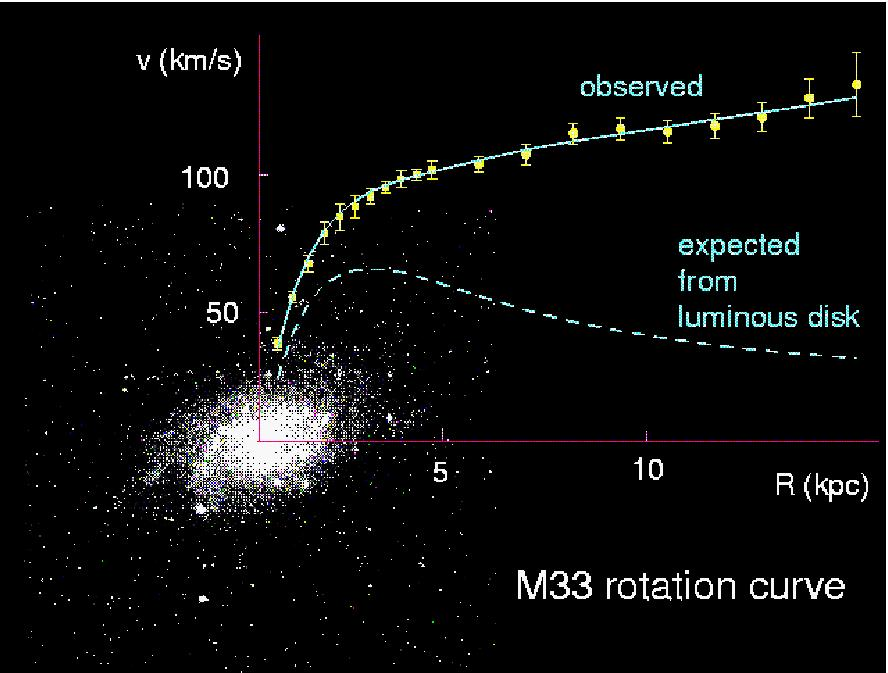
\includegraphics[width=5.5cm,height=4.cm]{rotationCurve.jpg}\\[-0.2cm] 
				\bl{   \fontF E.~Corbelli and P.~Salucci,   {\em Mon.\ Not.\ Roy.\ Astron.\ Soc.\  {\bf 311} 441}  (2000), %\\[-0.3cm]
					\href{https://arxiv.org/abs/astro-ph/9909252}{\fontF  arXiv:astro-ph/9909252}.}  
				\begin{textblock}{0.8}(0.94,1.5)
					\begin{turn}{70}
					{\bf \color{yellow} \Large Hint}
					\end{turn}
				\end{textblock}
				
				\column{0.5\textwidth}
				\vspace{-0.0cm}\centering 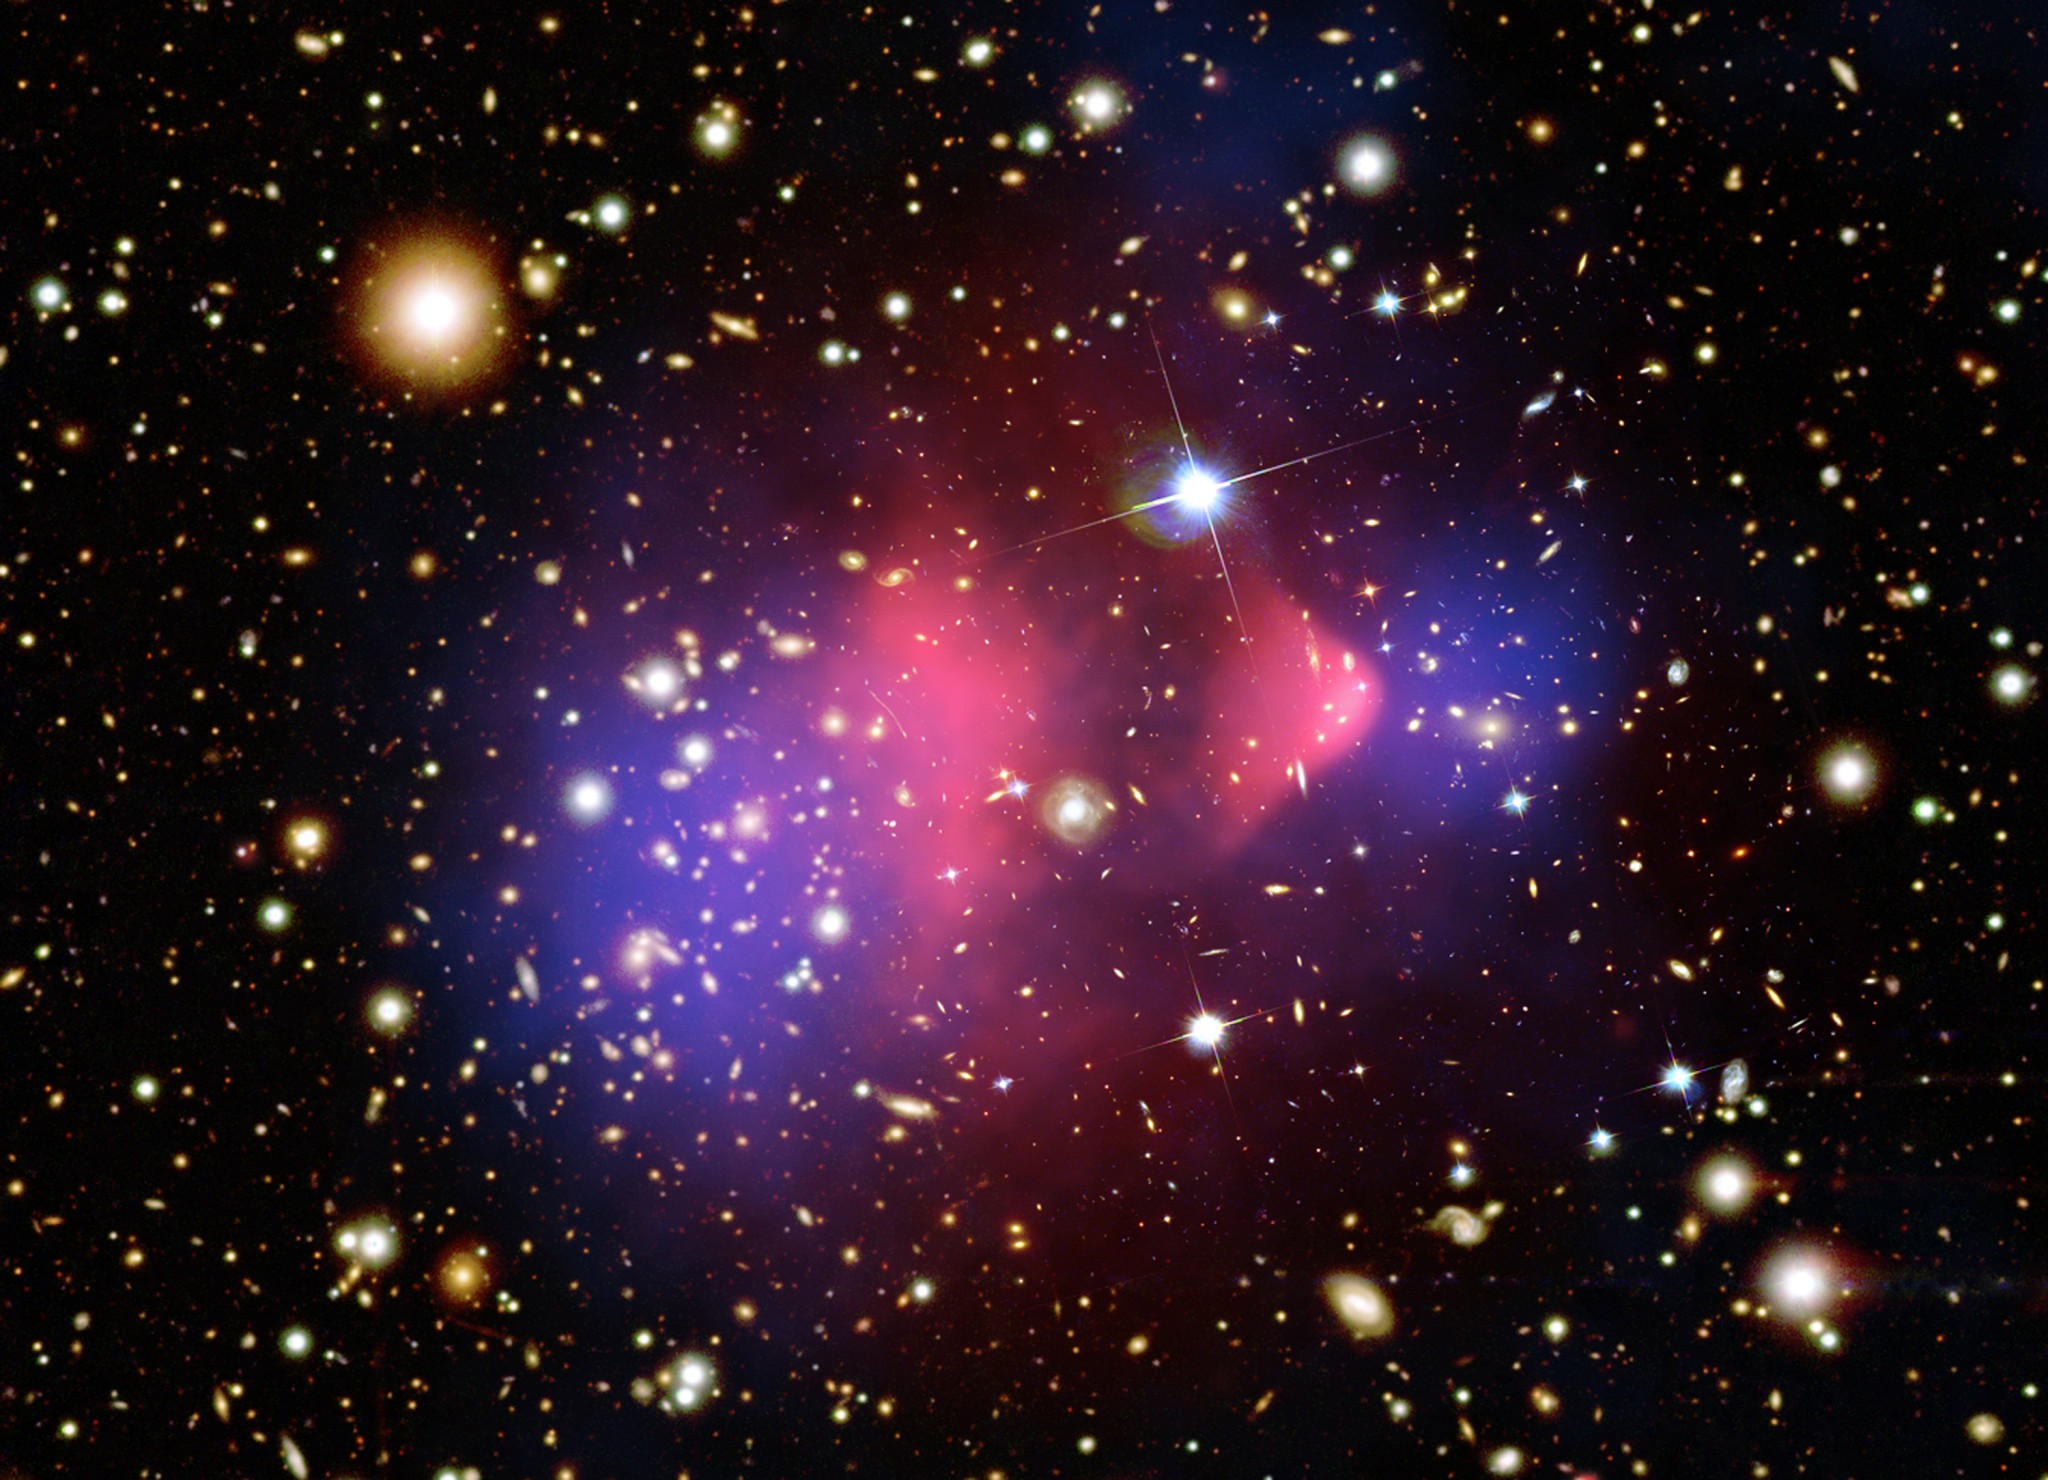
\includegraphics[width=5.5cm,height=4.cm]{BulletCluster.jpg} \\[-0.2cm] 
				\bl{ \fontF   M.~Markevitch, ESA Spec.\ Publ.\  {\bf 604} (2006) 723, \href{https://arxiv.org/abs/astro-ph/0511345}{\fontF  astro-ph/0511345}.%\\[-0.3cm] 
				  Clowe, Bradac, {\em  et. al.}  Astrophys.\ J.\  {\bf 648}, L109 (2006),    \href{https://arxiv.org/abs/astro-ph/0608407}{\fontF  astro-ph/0608407}           }
				
			\end{columns}
				\begin{textblock}{0.8}(8.4,1.5)
					\begin{turn}{70}
						{\bf \color{yellow} \Large Evidence}
					\end{turn}
				\end{textblock}
		
			\vspace*{-0.2cm}
			\begin{center}
				
				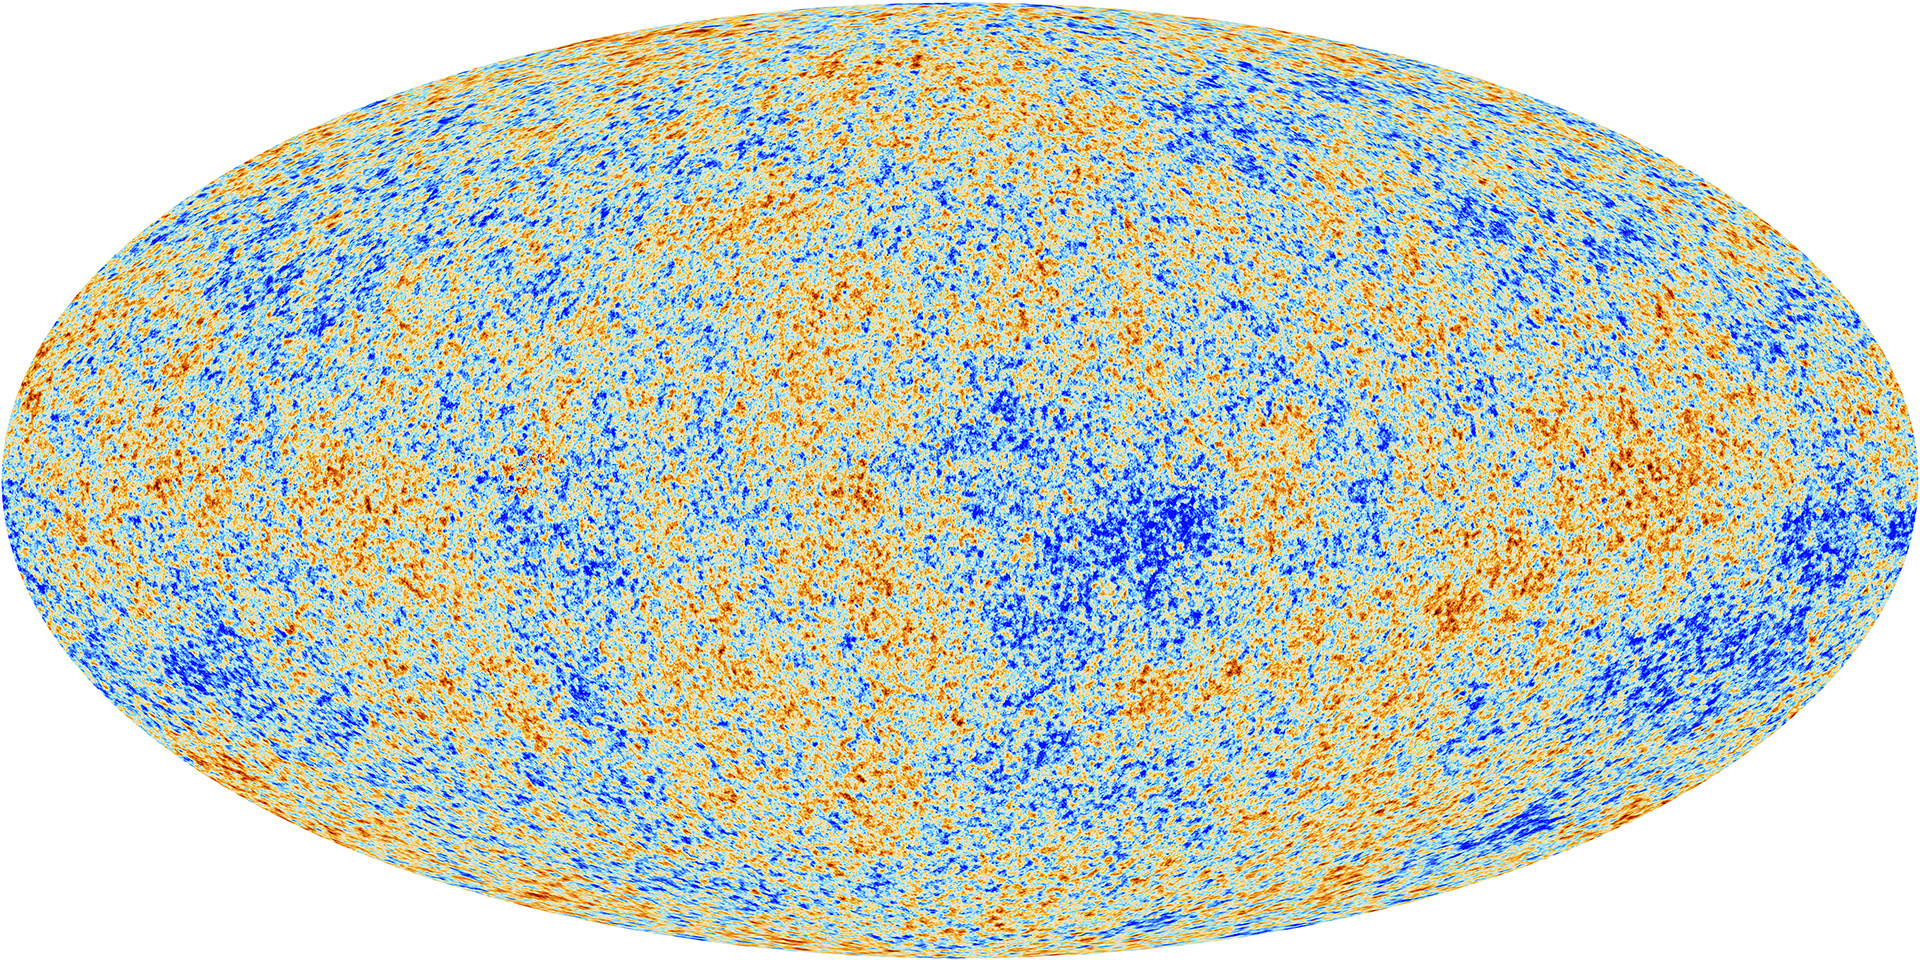
\includegraphics[width=6.cm, height=3.cm]{Planck_CMB.jpg}\\[-0.25cm] 
				\bl{ 
					\fontF  N.~Aghanim {\it et al.} [Planck Collaboration],
					%``Planck 2018 results. VI. Cosmological parameters,''
					\href{https://arxiv.org/abs/1807.06209}{\fontF  arXiv:1807.06209} [astro-ph.CO].
				}
			\begin{textblock}{0.8}(6.2,11.3)
%				$\Lambda$CDM
				\begin{turn}{0}
					{\color{black}  \Large $\Omega_{\rm DM}h^2 \approx 0.12$}
				\end{turn}
			\end{textblock}
			
			\end{center}	

		\end{frame}
%%%%%%%%%%%%%%%%%%%%%%%%%%%%%%%%%%%%%%%%%%%%%%%%%%%%%%%%%%%%%%%%%%%%%%%%%%%%%%%%%
\subsection{The dark matter particle}

%\vspace*{-6.5mm}    
%\begin{frame}{\insertsubsectionhead}
%	\hspace*{-11mm}
%	\includegraphics[width=\paperwidth]{You_Know_Nothing.jpg}
%\end{frame} 


%\newgeometry{margin=0pt}
%%%%%%%%%%%%%%%%%%%%%%%%%%%%%%%%%%%%%%%%%%%%%%%%%%%%%%%%%%%%%%%%%%%%%%%%%
\begin{frame}{\insertsubsectionhead}
	\begin{center}
		\begin{otherlanguage}{greek}
			<<Έν οἶδα, ὅτι οὐδὲν οἶδα.>>\\
		\end{otherlanguage}		
	``I know one thing,  that I know nothing."
	\flushright --Socrates \pause
	\end{center}

%	Properties:\pause
	\begin{itemize}
		\item Gravitational interactions.
		\item Mostly electrically neutral.
		\item Stable or very slow decay rate. 
		\item Non-Baryonic.
		\item Cold/Warm and non-relativistic today.
	\end{itemize}
	
\end{frame}
%%%%%%%%%%%%%%%%%%%%%%%%%%%%%%%%%%%%%%%%%%%%%%%%%%%%%%%%%%%%%%%%%%%%%%%%%

%%%%%%%%%%%%%%%%%%%%%%%%%%%%%%%%%%%%%%%%%%%%%%%%%%%%%%%%%%%%%%%%%%%%%%%%%
\subsection{The axion (like) particle}
\begin{frame}{\insertsubsectionhead}
%
Notably, the original Axion was originally introduced in order to solve the {\em strong-CP problem} of the SM.
Axion-Like-Particles (ALPs) arise in a number of new physics models, beyond the SM.  \\[0.5cm]

Axions and ALPs generally:
%
	\begin{itemize}
	\item Have suppressed interactions with photons.
	\item Are (mostly) stable. 
	\item Were non-relativistic around the epoch of structure formation. \pause
	\item Non-baryonic (by definition), and of-course interact gravitationally.\\[1cm]
\end{itemize}

\pause
\begin{center}
	{\bf \em Maybe DM has Axionic nature!}	
\end{center}

\end{frame}
%%%%%%%%%%%%%%%%%%%%%%%%%%%%%%%%%%%%%%%%%%%%%%%%%%%%%%%%%%%%%%%%%%%%%%%%%


%%%%%%%%%%%%%%%%%%%%%%%%%%%%%%%%%%%%%%%%%%%%%%%%%%%%%%%%%%%%%%%%%%%%%%%%%
\section{Calculating the Relic Abundance}
\subsection{The axion EOM}
\begin{frame}{\insertsubsectionhead}
	%
	Axions and ALPs follow a similar equation of motion (EOM):
	\begin{equation*}
		\lrb{\dfrac{d^2}{d t^2} + 3 H(t) \ \dfrac{d}{d t} } \theta(t) + \maT^2(t) \ \sin \theta(t) = 0 \; ,
	\end{equation*}	
	%
	where $\theta= A \, \fa$, with $A$ the axion filed, and $\fa$ some energy scale that characterises the potential (Peccei-Quinn breaking scale).


\end{frame}
%%%%%%%%%%%%%%%%%%%%%%%%%%%%%%%%%%%%%%%%%%%%%%%%%%%%%%%%%%%%%%%%%%%%%%%%%

%%%%%%%%%%%%%%%%%%%%%%%%%%%%%%%%%%%%%%%%%%%%%%%%%%%%%%%%%%%%%%%%%%%%%%%%%
\subsection{How hard can it be?}
\begin{frame}{\insertsubsectionhead}
	%
	\begin{center}
		\textbf{Hard} (in general).\\[1cm]\pause
	\end{center}	

	The classical analogue is the dumped pendulum with both frequency (length) and friction being time-dependent:
	%
	\begin{itemize}
		\item There is no closed form solution.
		\item There are no constants of motion (wait a minute).
		\item No package/library/program available!\\[2cm]\pause
	\end{itemize}

	\begin{center}
		{\sl \mimes simulates the evolution of the Axion/ALP, for (virtually) any cosmological scenario and Axion/ALP (thermal) mass.}
	\end{center}		
\end{frame}
%%%%%%%%%%%%%%%%%%%%%%%%%%%%%%%%%%%%%%%%%%%%%%%%%%%%%%%%%%%%%%%%%%%%%%%%%

%%%%%%%%%%%%%%%%%%%%%%%%%%%%%%%%%%%%%%%%%%%%%%%%%%%%%%%%%%%%%%%%%%%%%%%%%
\subsection{Initial conditions}
\begin{frame}{\insertsubsectionhead}
	%
	Some time at the very early Universe, $\maT \ll H(T)$,~\footnote{\fontF This is an assumption that \mimes has to make, for the sake of generality.} with
	\begin{equation*}
		\ddot{\theta}  + 3H \ \dot{\theta} \approx 0 \;.
	\end{equation*}	
	%
	The solution is 
	$$
	\theta = \thetai + C \dint_{0}^t d t' \ \lrb{ \dfrac{a(t'=0)}{a(t')} }^3 \;.
	$$
	%this is true especially in the case where the PQ symmetry breakes before inflation.
	So, $\dot{\theta} \sim a^{-3}$. Since we are interested in $\theta$ at much later times (once the potential becomes relevant), $\dot{\theta} \approx 0$.~\footnote{\fontF Standard misalignment mechanism. For the kinetic one see
	%
	\bl{\fontF R.~T.~Co, L.~J.~Hall and K.~Harigaya,
		\href{https://doi.org/10.1103/PhysRevLett.124.251802}{Phys. Rev. Lett. \textbf{124} (2020) no.25, 251802}
		\href{https://arxiv.org/abs/1910.14152}{[arXiv:1910.14152 [hep-ph]]}},
	%
	\bl{\fontF  C.~F.~Chang and Y.~Cui,
		\href{https://doi.org/10.1103/PhysRevD.102.015003}{Phys. Rev. D \textbf{102} (2020) no.1, 015003}
		\href{https://arxiv.org/abs/1911.11885}{[arXiv:1911.11885 [hep-ph]]}}, or 
	% 
	\bl{\fontF  B.~Barman, N.~Bernal, N.~Ramberg and L.~Visinelli,
		\href{https://arxiv.org/abs/2111.03677}{[arXiv:2111.03677 [hep-ph]]} }.	
	}
	%
	Therefore, we can start integration at some point ($t=\ti$) with $3H \gg \maT$, and set $\theta(t=\ti) = \thetai$ and $\dot \theta(t=\ti) = 0$. 

\end{frame}
%%%%%%%%%%%%%%%%%%%%%%%%%%%%%%%%%%%%%%%%%%%%%%%%%%%%%%%%%%%%%%%%%%%%%%%%%
\subsection{(Bad) Analytical approximations}
\begin{frame}{\insertsubsectionhead}
	Once we agree on the initial conditions, we move to the next important things:\pause
	%	
	%\begin{equation*}
	%	\ddot \theta + \underbrace{  \bl{ 3\overbrace{H(t) }^{\text{Slow}}  } \ \dot \theta + \bl{ \overbrace{\maT^2(t)}^{\text{Slow}}  }}_{\maT > 3 H} \ \rd{\underbrace{ \sin \theta(t) }_{\theta \ll 1}  } = 0 \; ,
	%\end{equation*}	
	%
	\begin{itemize}
		\item Assume $\theta \ll 1$, and linearise the EOM. {\sl Not always that bad.}\pause
		\item Assume that at $\maT(\Tosc) \approx 3H(\Tosc)$, the oscillations begin with $\dot\theta(\Tosc)=0$. {\sl This is in general quite bad.}\pause
		\item Assume that $\thetaosc \approx \thetai$. {\sl Generally quite bad.}\pause
	\end{itemize}
	
	Then, we get the ``WKB"-approximate solution
	%
	\begin{equation*}\vspace*{-0.2cm}
	\theta(t) \approx \thetai \lrb{\dfrac{3}{4}}^{1/4} \sqrt{ \dfrac{ \maT(\Tosc) }{\maT(T)} } \lrb{\dfrac{a}{\aosc}}^{-3/2} \  \cos\lrb{ \int_{\tosc}^t d t^\prime  \ \maT(t^\prime)}   \;.
	\end{equation*}
	
	The advantage of this approximation is that we get an easy formula for the axion/ALP energy density today:
	%
	\begin{equation*}\vspace*{-0.2cm}		
		\rho_{a,0} = \gamma^{-1}  \dfrac{s_0}{s_{\rm osc}} \  \dfrac{1 }{2}  \ \fa^2 \ \ma \ \maT_{,{\rm osc}} \ \thetai^2    \;,
	\end{equation*}
	%
	where $\gamma$ the amount of entropy injection between $\Tosc$ and today.~\footnote{\fontF Defined from $s(T_0) = \gamma \ \aosc^3 \ s_{\rm osc}$.}
\end{frame}

%%%%%%%%%%%%%%%%%%%%%%%%%%%%%%%%%%%%%%%%%%%%%%%%%%%%%%%%%%%%%%%%%%%%%%%%%
%\subsection{I feel a need... need for accuracy (and speed)}
\subsection{Need for accuracy, speed, and automation}
\begin{frame}{\insertsubsectionhead}
	%
	Serious disadvantages of the approximate results:
	% 
	\begin{itemize}
		\item The approximations can be tested against numerical results in a case-by-case basis; there is no way to tell if they will work in new models and cosmological scenarios.
		\item There is no available tool that can help us reproduce published results obtained by numerical integration; people use their own {\bf \em private} code. %peer-review process?
		\item If someone wants to simply see if an ALP model is compatible with a cosmological scenario, they have to develop their own private code; the overall effort of the community increases.
	\end{itemize}

	\mimes:
	% 
	\begin{itemize}
		\item {\sl Easy} to use; anyone can run it and see if their model can work.
		\item Reasonably fast; less than $0.05 \; s$ for the scenarios tested.
		\item Tools that can help determine if the algorithm is accurate enough.
		\item The user provides too much input. This helps the user determine whether convergence of the algorithm is consistent. 
	\end{itemize}

\end{frame}


%%%%%%%%%%%%%%%%%%%%%%%%%%%%%%%%%%%%%%%%%%%%%%%%%%%%%%%%%%%%%%%%%%%%%%%%%
\section{\mimes}
\subsection{\mimes: General}
\begin{frame}{\insertsubsectionhead}
%
%From the software point of view:\pause
%
\begin{itemize}
	\item \mimes is a \CPP header-only library that contains various templated classes; there is no ``installation" and no special procedures, just include the header files. \pause
	%
	\item \mimes comes with a \PY interface so that everybody can use it.\pause
	%
	\item \mimes is distributed under the MIT license; you can do whatever you want with it, and I am {\em not} responsible.\pause
\end{itemize}


\end{frame}
%%%%%%%%%%%%%%%%%%%%%%%%%%%%%%%%%%%%%%%%%%%%%%%%%%%%%%%%%%%%%%%%%%%%%%%%%
\subsection{\mimes: Under the hood}
\begin{frame}{\insertsubsectionhead}
	%
	\mimes relies on \cppin{NaBBODES}~\footnote{\fontF \href{https://github.com/dkaramit/NaBBODES}{https://github.com/dkaramit/NaBBODES}.} for the numerical integration, and \cppin{SimpleSplines}~\footnote{\fontF \href{https://github.com/dkaramit/SimpleSplines}{https://github.com/dkaramit/SimpleSplines}.} for the various interpolations.\\[0.3cm] 
	
	Advantages:
	%
	\begin{itemize}
		\item You only need to have the standard \CPP library.
		\item The two libraries are developed by myself, so their integration with \mimes is seamless.
		\item There is always going to be a compatible version of these libraries that works with \mimes.\\[0.3cm]
	\end{itemize}	
	
	Disadvantages:
	%
	\begin{itemize}
		\item These are not well tested libraries.
		\item No community of contributors; if it doesn't work, I have to fix it.
		\item Slow development.
	\end{itemize}	

\end{frame}
%%%%%%%%%%%%%%%%%%%%%%%%%%%%%%%%%%%%%%%%%%%%%%%%%%%%%%%%%%%%%%%%%%%%%%%%%
\subsection{\mimes: Notation}
\begin{frame}{\insertsubsectionhead}
	%
	\vspace{-0.2cm}
	\mimes uses a notation suitable (any) underlying cosmology, since it is up to the user to define the cosmological evolution.	
	First, we define 
	\begin{equation*}\vspace{-0.2cm}
		u \equiv \log \lrb{a/\ai}\;,
	\end{equation*} 
	%
	with $\ai$ some initial value of the scale factor.~\footnote{\fontF Only the ratios $a/\ai$ appear in the calculations. So, the choice does not matter as long as it is consistent.} in order to express the time derivatives as 
	%
	\begin{equation*}
		\dfrac{d  }{dt}  \to  H  \dfrac{d }{du} \;, 
		 \quad
		\dfrac{d^2 }{dt^2}  \to H^2 \ \lrb{ \dfrac{d^2 }{du^2} + \dfrac{1}{2} \dfrac{d \log H^2}{du}  \dfrac{d }{du} }\;.
	\end{equation*}
	%
	Then, we express the EOM as a system of first order ordinary differential equations
	%
	\begin{eqnarray*}\vspace*{-0.5cm}
		& \dfrac{d  \zeta}{du} + \lrsb{\dfrac{1}{2} \dfrac{d \log H^2}{du} + 3 } \zeta + \ \lrb{\dfrac{\maT}{H}}^2 \ \sin \theta
		=0 \;. \\[-0.2cm]
		&\dfrac{d \theta}{d u} - \zeta=0 \;.
	\end{eqnarray*}\\[-0.2cm]
	%
	Observe that, by definition, $\zeta = d\theta / du$. The initial conditions are $\zeta(0)=0$ and $\theta(0)=\thetai$.
	
\end{frame}
%%%%%%%%%%%%%%%%%%%%%%%%%%%%%%%%%%%%%%%%%%%%%%%%%%%%%%%%%%%%%%%%%%%%%%%%%
\subsection{\mimes: When do you start and stop integrating?}
\begin{frame}{\insertsubsectionhead}
	%
	The choice of a good starting point is important, as need to start at a temperature where $\zeta=0$ is a good approximation. So you can start at some $\Ti$ with a given ratio $3H(\Ti)/\maT(\Ti) \gg 1$.  This needs to be chosen carefully, as low values of $3H(\Ti)/\maT(\Ti)$ result in inaccurate result, while high values may result in a slow calculation. {\sl Advice}: Use various values of that ratio, and find where the relic abundance becomes $\Ti$-independent.\\[0.5cm]
	
	The stopping condition is more difficult. You should stop at some point where the axion/ALP evolves "adiabatically". Find a quantity that becomes constant as the system relaxes, and use this to determine when adiabaticity is reached. Once $\theta$ starts to evolve adiabatically, the amplitude of its oscillation is known at later times!
\end{frame}
%%%%%%%%%%%%%%%%%%%%%%%%%%%%%%%%%%%%%%%%%%%%%%%%%%%%%%%%%%%%%%%%%%%%%%%%%
\subsection{\mimes: Some (classical) physics}
\begin{frame}{\insertsubsectionhead}
	%
	If a system exhibits closed orbits, the quantity
	%
	\begin{equation*}
		J \equiv C \ \oint p \ d \theta \;,
	\end{equation*}
	%
	is the adiabatic invariant. In this case, it becomes
	%
	\begin{equation*}
		J = a^3 \ \maT \ \thetamax^2  \, f(\thetamax)  \;,
	\end{equation*}
	%
	with 
	\begin{equation*}
		f(\thetamax) =\dfrac{ 2 \sqrt{2}}{\pi \thetamax^2 } \dint_{- \thetamax}^{\thetamax} d \theta \sqrt{ \cos \theta - \cos \thetamax } \;,
	\end{equation*}
	 %
	 the so-called anharmonic factor.\pause
		 
	\textbf{Important}: $\thetamax$ is the peak of the oscillation. So, $J$ can be used to determine how $\thetamax$ changes with time. By definition, at $\theta=\thetamax$, $p \sim \dot \theta = 0$.
	This means that we can find $\rho_{a,0}$ on the peak of today's $\theta$, as
	%
	\begin{equation*}
		\rho_{a,0} = \gamma^{-1} \ \dfrac{s_0}{s_*} \ \ma \ \maT_{,*} \ \dfrac{1}{2} \ \fa^2 \ \thetamax_{,*}^2 \;  \ f(\thetamax_{,*}) \;,
	\end{equation*}
	%
	where $T_{*}$ the temperature at which adiabaticity was reached, and $\gamma$ the entropy injection between $T_*$ and today (\ie $s_0 = \gamma a_*^3 s_*$). 	  
\end{frame}

\section{Using \mimes}

\subsection{How to get \mimes}
\begin{frame}[fragile]{\insertsubsectionhead}
	There are several ways you can get a stable version of \mimes:
	\begin{enumerate}
		%
		\item \cppin{git clone -b stable https://github.com/dkaramit/MiMeS.git}. This is the preferred way, as it is guaranteed to be the latest stable version.
		%
		\item Go to \href{https://mimes.hepforge.org/downloads}{mimes.hepforge.org/downloads}, and download it. 
		%
		\item Go to \href{https://github.com/dkaramit/MiMeS/releases}{github.com/dkaramit/MiMeS/releases}, and download a released version.    
	\end{enumerate}

	
	You can get the most up-to-date code -- not always the most stable one -- including the latest version of {\tt NaBBODES} and {\tt SimpleSplines}, by running
	%
	\begin{lstlisting}
		git clone https://github.com/dkaramit/MiMeS.git
		cd MiMeS
		git submodule init
		git submodule update --remote
	\end{lstlisting}

\end{frame}

\subsection{Configure (and make)}
\begin{frame}[fragile]{\insertsubsectionhead}
	There is no need to install anything if you are going to use \mimes in a \CPP program. The only thing you {\em must} do is run 
	\begin{bash}
		bash configure.sh
	\end{bash}
	%	
	Alter that, you can include the header file \cppin{MiMeS/MiMeS.hpp}, and you are good to go.
	
	However, you can also run 
	%
	\begin{itemize}
		\item \cppin{make lib}, in order to produce the (shared) libraries. This is needed in order to run the \PY interface. 
		\item \cppin{make examples}, in order to compile the examples in \cppin{MiMeS/UserSpace/Cpp}.
		\item \cppin{make exec}, in order to produce some test executables  (in \cppin{MiMeS/exec}). You just need to run then in order to see if you get any segfaults.
	\end{itemize}
\end{frame}


\subsection{Classes}
\begin{frame}[fragile]{\insertsubsectionhead}
	There are three classes useful to the user.~\footnote{\fontF There are various arguments that need to be passed to the constructors, and the are all listed and explained in the Appendix of the documentation.}
	%
	\begin{itemize}
	\item \cppin{mimes::Cosmo<LD>}: interpolation of relativistic degrees of freedom of the plasma. By default it uses the EOS2020~\footnote{\fontF 
		\bl{K.~Saikawa and S.~Shirai,
		\href{https://doi.org/10.1088/1475-7516/2020/08/011}{JCAP \textbf{08} (2020), 011}
		\href{https://arxiv.org/abs/2005.03544}{[arXiv:2005.03544 [hep-ph]]}.}
	} data. The user can choose another file easily.
	%
	\pause
	%
	\item \cppin{mimes::AxionMass<LD>}: definition of axion/ALP mass as a function of the temperature and $\fa$. \mimes is shipped with data from Lattice calculation~\footnote{\fontF \bl{
			S.~Borsanyi, Z.~Fodor, J.~Guenther, K.~H.~Kampert, S.~D.~Katz, T.~Kawanai, T.~G.~Kovacs, S.~W.~Mages, A.~Pasztor and F.~Pittler, \textit{et al.}
			\href{https://doi.org/10.1038/nature20115}{Nature \textbf{539} (2016) no.7627, 69-71}
			\href{https://arxiv.org/abs/1606.07494}{[arXiv:1606.07494 [hep-lat]]}.}} of the QCD axion mass.
	 %
	 \pause
	%	
	\item \cppin{mimes::Axion<LD,Solver,Method>}: This is responsible for actually solving the EOM.
	\end{itemize}
	
	
\end{frame}

\subsection{Assumptions}
\begin{frame}[fragile]{\insertsubsectionhead}
	
	\mimes is designed to make as few assumption as possible. However, it still assumes that:\pause
	%
	\begin{enumerate}
		\item $H/\maT$ increases monotonically with the temperature.\pause
		\item $\zeta(0)=0$. This will be changed in the future.\pause
		\item The energy density of the axion/ALP is always subdominant.\pause
		\item Only the EOM determines the energy density (no annihilations, no strings, etc.).
	\end{enumerate}
	
	
\end{frame}


\subsection{What \mimes expects from you}
\begin{frame}[fragile]{\insertsubsectionhead}
	Apart from $\thetai$ and $\fa$, keep in mind that \mimes needs:
	%
	\begin{enumerate}
		\item The mass of the axion/ALP. A data file or an actual function.
		\item Data file with $\log a/a_i$ ($a_i$ is some arbitrary value; \mimes rescales it appropriately), $T$, and $\log H$ of the underlying cosmology.\pause
		\item Value for $3H/\maT \gg 1$, which defines the point where integration begins.\pause
		\item Relative difference of $J$ between a given number of peaks at which we consider adiabaticity to have been reached.\pause
		\item Other input, related to the algorithm, that might confuse you; \eg temperature at which integration stops no {\em matter what}!
	\end{enumerate}
\end{frame}


\subsection{Template arguments}
\begin{frame}[fragile]{\insertsubsectionhead}
	%
	You need to choose what numeric type to use. This is done by the template argument \cppin{LD} which should be \cppin{double} (fast) or \cppin{long double} (accurate).~\footnote{\fontF You could choose \cppin{float}, but we live in 2021.}\\[0.5cm]
	
	
	You also need to tell \mimes which integration strategy to use. This is done by choosing template arguments:
	%
	\begin{itemize}
		\item \cppin{Solver} can be set to \cppin{1} for Rosenbrock (semi-implicit Runge-Kutta). 
		The \cppin{Method} argument in this case can be:\\[-0.0cm]
		\begin{itemize}
			\item \cppin{RODASPR2<LD>} (4th order).
			\item \cppin{ROS34PW2<LD>} (3rd order).
			\item \cppin{ROS3W<LD>} (2rd order, {\em very} bad).
		\end{itemize}
		\item \cppin{Solver} can be set to \cppin{2} for explicit RK.
		The \cppin{Method} argument can be:\\[-0.0cm]
		\begin{itemize}
			\item \cppin{DormandPrinceRK45<LD>} (7th order)
			\item \cppin{CashKarpRK45<LD>} (5th order, {\em very} bad).
			\item \cppin{RK45<LD>} (5th order, {\em very} bad).
		\end{itemize}	
	\end{itemize}
\end{frame}

\subsection{\mimes from \PY}
\begin{frame}[fragile]{\insertsubsectionhead}
	In order to call the \PY interface of \mimes, we need to first call \cppin{make lib} in the root directory of \mimes.\\[0.2cm]
	
	Before that, we can take some time to decide what the template arguments and compilation  options should be. In the 
	file \cppin{MiMeS/Definitions.mk}, you can change the variables:
	%
	\begin{itemize}
		\item \cppin{LONG=long} will compile the library with \cppin{long double} numeric types. \cppin{LONG=} will compile the library with \cppin{double} numeric types.
		\item \cppin{SOLVER} and \cppin{METHOD}, as in the template arguments.
	\end{itemize}
	
	Also, in the same file, you can change compilation options:
	%
	\begin{itemize}
		\item Compiler:
		\begin{itemize}
			\item \cppin{CC=g++} in order to use the \cppin{GNU} \CPP compiler.
			\item \cppin{CC=clang -lstdc++} in order to use the \cppin{clang} \CPP compiler.
		\end{itemize}
	\item Optimization level:
		\begin{itemize}
			\item \cppin{OPT=O0}: No optimization. 
			\item \cppin{O=O1}, \cppin{O2}, or \cppin{O3} (marginally faster, default): some optimization occurs (read the compiler documentation for more information).
			\item \cppin{OPT=Ofast}: full optimization (fast, but dangerous). 
		\end{itemize}
	\end{itemize}
\end{frame}


\section{Examples}
\subsection{\CPP}
\begin{frame}[fragile]{\insertsubsectionhead}
	Define everything and solve in just a few lines of code!\\[0.3cm]
	\lstset{language = c++}
	\lstinputlisting[basicstyle=\fontF]{example.cpp}
\end{frame}

\subsection{\PY}
\begin{frame}[fragile]{\insertsubsectionhead}
\end{frame}

\section{Outlook}

\subsection{Summing up}
\begin{frame}[fragile]{\insertsubsectionhead}
	\DK{blah blah, what you did}
\end{frame}

\subsection{Future}
\begin{frame}[fragile]{\insertsubsectionhead}
	\DK{Freeze-out/in, kinematic misalignment mechanism, automatically compare with searches.}
\end{frame}


\setbeamercolor{structure}{fg=black!80!red}
\setbeamercolor{section in head/foot}{fg=white, bg=red}
\setbeamertemplate{footline}{
	%\begin{beamercolorbox}[wd=1\textwidth,ht=2.25ex,dp=1ex,right]{section in head/foot}%
		%\insertsubsectionhead 
		%\insertframenumber/\inserttotalframenumber
		%\end{beamercolorbox}
}
\setbeamertemplate{background canvas}{%
	
\begin{tikzpicture}[remember picture,overlay]
		\shade[left color=red!90!black, right color=black!80!red]
		([shift={(0.0cm,-0.0cm)}]current page.north west)
		rectangle
		([shift={(-0.0cm,0.0cm)}]current page.south east);
	\end{tikzpicture}%     
}
%\setbeamercolor{background canvas}{bg=red}
\begin{frame}[noframenumbering]
	
	\begin{center}
		{\color{yellow} \Huge Thank you!}
		\begin{figure}
			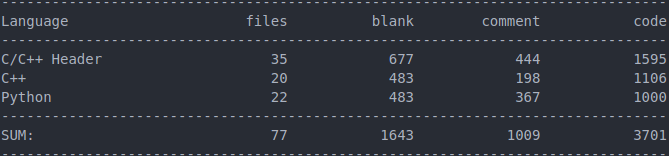
\includegraphics[width=1\textwidth]{cloc.png}
		\end{figure}	

	\end{center}
\end{frame}



\setbeamertemplate{background canvas}{%
	
\begin{tikzpicture}[remember picture,overlay]
		\shade[left color=black!90!red, right color=red!80!black]
		([shift={(0.0cm,-0.0cm)}]current page.north west)
		rectangle
		([shift={(-0.0cm,0.0cm)}]current page.south east);
	\end{tikzpicture}%     
}

%%Put equations for Back-up. 
\begin{frame}[noframenumbering]
	%	
	\begin{center}
		{\color{yellow} \Huge Backup \\ {\tiny (equations, derivations, tables)}}
	\end{center}
	%	
\end{frame}
%
\setbeamertemplate{background canvas}{}
\setbeamercolor{background canvas}{bg=white}

\begin{frame}{WKB}
	
\end{frame}

\begin{frame}{Adiabatic invariant}
	
\end{frame}

\begin{frame}{Input -- \cppin{mimes::AxionMass<LD>}}
	
\end{frame}

\begin{frame}{Input -- \cppin{mimes::Axion<LD,Solver,Method>}}
	
\end{frame}






\end{document}